%!TeX root=../tese.tex
%("dica" para o editor de texto: este arquivo é parte de um documento maior)
% para saber mais: https://tex.stackexchange.com/q/78101

% Aqui podemos começar falando um pouco sobre o background de explainable AI e depois conectamos
% falando sobre redes neurais e gradiente descendente para, por fim, falar um pouco sobre CNNs.


\enlargethispage{-1\baselineskip}

\chapter{Background}

In this chapter, we will introduce important concepts required for the understanding of this study.
We begin by introducing Explainable AI (XAI) and its principles. We also introduce Neural Networks and important concepts such as Gradient Descent and Back Propagation. 
Finally, we introduce Convolutional Neural Networks, the main focus of this study.

\section{Explainable AI}

With the rise of Machine Learning models in the last decade in the business and academic areas, Artificial Intelligence (AI) is becoming increasingly present in important decision-making tasks. 
However, as AI models have become more sophisticated, particularly with the advent of Deep Learning techniques, their internal workings have often remained opaque. 
Explainable AI (XAI) aims to make models and their decisions more transparent, interpretable and understandable to both experts and inexperienced users.

\subsection{What is Explainable AI?}

Defining a mathematical formalization to explainability of Machine Learning is a difficult task considering the subjective nature of what one may consider "explainable". In non-mathematical terms, 
Explainability in AI refers to the capacity to articulate or justify the behavior of a model, focusing on methods that explain a model's decisions after they are made.

Another important concept in the area is Interpretability, which can be defined as "the degree to which a human can understand the cause of a decision" by Miller (2017)\footnote[1]{Miller, Tim. “Explanation in artificial intelligence: Insights from the social sciences.” arXiv Preprint arXiv:1706.07269. (2017).}.
In this case, however, a model's decision is understandable entirely by its inherent transparency. In other terms, the model is simple enough to be interpretable by a human directly, without the use of external techniques.

Models with low complexity whose decisions are understandable by humans are defined as \emph{Interpretable Models}. Linear Regression, Logistic Regression and Decision Tree models are examples of models classified as \emph{Interpretable Models}. 
Now, models with a level of complexity that prevents humans from directly understanding their decision-making processes are referred to as \emph{Explainable Models}. 
Recently popular \emph{Deep Learning Models} are one kind of \emph{Explainable Models} and will be the main focus of this essay, especially \emph{Deep Convolutional Neural Networks}, explored in \hyperref[sec:convolutions]{section 1.3}.
% CUIDADO AQUI EM CIMA!!! PODE MUDAR O NÚMERO DA SESSÃO

\subsection{Why Explainable AI is Necessary}

Creating explanations to a model's decisions can yield many advantages, including increase in model trust, more ethical and fair decisions, correctly following regulatory compliances and easier model debugging.

While Debugging, Machine Learning models can have quite unpredictable behavior, detecting biases not initially noticed by humans. This can yield great performance in the training or even validation and test datasets,
but poor performance in real world deployment. For example, while training an image classifier on dog and cat images one can find great accuracy on classification of dogs over green fields. However, 
when analyzing what regions of the image a model "sees" for the prediction, researchers may find out that the model is actually looking at the image background, 
since dog owners tend to take their pets for walks more often than cat owners, therefore making dog pictures with a green background more likely than pictures with cats over green fields. 
Visualizing regions of images that our vision model "sees" is only possible with Explainable AI techniques, such as GradCAM (\emph{COLOCAR REFERÊNCIA AQUI}) and other Gradient Saliency methods.

\cite{zobel:04}


\section{Gradient Descent}

Let \(f\colon A \to B\) where \(A \subseteq \mathbb{R}^n\) for \(n \in \mathbb{N}\) and \(B \subseteq \mathbb{R^+}\). Suppose we want to find the solution to the optimization problem

\[\argmin_{x \in A} f(x)\]
when \(\frac{\partial f}{\partial x}\) is known for any value of \(x\). Considering that the vector \(\frac{\partial f}{\partial x}\) points to the direction of the steepest ascent of the function, the vector \(- \frac{\partial f}{\partial x}\) will point to the steepest descent from the given point \(x\).
Therefore, one can define an initial random value for \(x\) and update \(x\) using \(- \frac{\partial f}{\partial x}\) and a scaling factor \(\eta\) in order to find a local minimum of \(f\) and an approximation to the solution of given optimization problem.

We can define such method using the following formula, where \(x_t\) represents the value of \(x\) at iteration \(t\) of the algorithm:

\[x_{t + 1} = x_t - \eta \frac{\partial f}{\partial x}.\]

The term \(\eta\) is often called the \emph{learning rate} used in the Gradient Descent method and is often defined manually by the user.

The Gradient Descent method can be used to optimize a neural network's parameters to solve a given problem using a \emph{loss function}. 
% TODO: Devo adicionar menção que vamos usar isso também com Feature Visualization?

\section{Neural Networks}

Neural Networks are proven to be universal approximators\footnote{Hornik, K., Stinchcombe, M., White, H. Multilayer feedforward networks are universal approximators. https://doi.org/10.1016/0893-6080(89)90020-8}. That means that Neural Networks are Machine Learning models capable of representing any continuous function,
therefore making Neural networks adept at modeling a range of different complex problems.
This class of models have seen a growing presence across both academic and industry landscapes. However, given the architecture of multiple hidden layers of Neural Networks creating complex internal patterns, such models are classified as Explainable Models. 

In this section, the inner workings of Neural Networks will be explained, starting with the \emph{Perceptron}, considered the fundamental building block of Neural Networks.

\subsection{Perceptron}

A Perceptron is a Machine Learning model inspired by how biological neurons work. 
It is a simple binary linear classifier that defines its parameters by linear combinations of points in the dataset.
The Perceptron model can be described by Figure \ref{fig:perceptron}. 

\begin{figure}
    \centering
    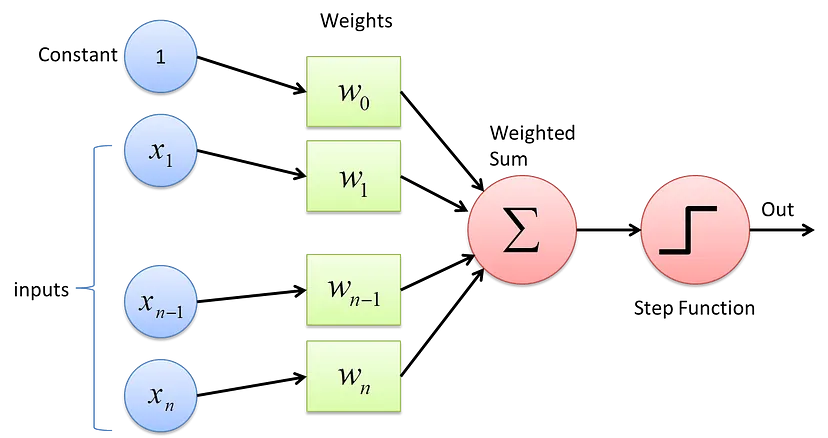
\includegraphics[scale=0.4]{figuras/perceptron.png}
    \caption{Perceptron Architecture. Font: \emph{Towards Data Science\footnotemark}. \label{fig:perceptron}}
\end{figure}
\footnotetext{https://towardsdatascience.com/what-the-hell-is-perceptron-626217814f53}

Where the weights \(w_i\) for \(i \in \{0, 1, \cdots, n\}\) are trainable parameters and the step function can be defined as \(\sigma \colon \mathbb{R} \to \{0, 1\}\) such that

\[\sigma(x) = 
\begin{cases}
    1 & \text{ if } x \geq 0 \\
    0 & \text{ if } x < 0.
\end{cases}\]

Therefore, the Perceptron model can be defined as the function \(f \colon \mathbb{R}^n \to \{0, 1\}\) where

\[f(x) = \sigma(w_0 + \sum_{i = 1}^{n} w_i x_i).\]

The Perceptron model updates its parameters using each sample \((x, y)\) of the dataset with the rule

\[w_i^{t + 1} = w_i^t + \eta \; (y - f(x)) x_i\]
for \(i \in \{1, \cdots, n\}\) and

\[w_0^{t + 1} = w_0^t + \eta \; (y - f(x)),\]
where \(\eta\) is the \emph{learning rate} hyperparameter and \(t\) is the update iteration number.

As a linear model, the Perceptron can only model linear problems. 
\section{Convolutional Neural Networks}
\label{sec:convolutions}

\lipsum[5-6]



